% Options for packages loaded elsewhere
\PassOptionsToPackage{unicode}{hyperref}
\PassOptionsToPackage{hyphens}{url}
\PassOptionsToPackage{dvipsnames,svgnames,x11names}{xcolor}
%
\documentclass[
  sn-basic,
]{sn-jnl}



\usepackage{amsmath,amssymb}
\usepackage{iftex}
\ifPDFTeX
  \usepackage[T1]{fontenc}
  \usepackage[utf8]{inputenc}
  \usepackage{textcomp} % provide euro and other symbols
\else % if luatex or xetex
  \usepackage{unicode-math}
  \defaultfontfeatures{Scale=MatchLowercase}
  \defaultfontfeatures[\rmfamily]{Ligatures=TeX,Scale=1}
\fi
\usepackage{lmodern}
\ifPDFTeX\else  
    % xetex/luatex font selection
\fi
% Use upquote if available, for straight quotes in verbatim environments
\IfFileExists{upquote.sty}{\usepackage{upquote}}{}
\IfFileExists{microtype.sty}{% use microtype if available
  \usepackage[]{microtype}
  \UseMicrotypeSet[protrusion]{basicmath} % disable protrusion for tt fonts
}{}
\makeatletter
\@ifundefined{KOMAClassName}{% if non-KOMA class
  \IfFileExists{parskip.sty}{%
    \usepackage{parskip}
  }{% else
    \setlength{\parindent}{0pt}
    \setlength{\parskip}{6pt plus 2pt minus 1pt}}
}{% if KOMA class
  \KOMAoptions{parskip=half}}
\makeatother
\usepackage{xcolor}
\setlength{\emergencystretch}{3em} % prevent overfull lines
\setcounter{secnumdepth}{5}
% Make \paragraph and \subparagraph free-standing
\ifx\paragraph\undefined\else
  \let\oldparagraph\paragraph
  \renewcommand{\paragraph}[1]{\oldparagraph{#1}\mbox{}}
\fi
\ifx\subparagraph\undefined\else
  \let\oldsubparagraph\subparagraph
  \renewcommand{\subparagraph}[1]{\oldsubparagraph{#1}\mbox{}}
\fi


\providecommand{\tightlist}{%
  \setlength{\itemsep}{0pt}\setlength{\parskip}{0pt}}\usepackage{longtable,booktabs,array}
\usepackage{calc} % for calculating minipage widths
% Correct order of tables after \paragraph or \subparagraph
\usepackage{etoolbox}
\makeatletter
\patchcmd\longtable{\par}{\if@noskipsec\mbox{}\fi\par}{}{}
\makeatother
% Allow footnotes in longtable head/foot
\IfFileExists{footnotehyper.sty}{\usepackage{footnotehyper}}{\usepackage{footnote}}
\makesavenoteenv{longtable}
\usepackage{graphicx}
\makeatletter
\def\maxwidth{\ifdim\Gin@nat@width>\linewidth\linewidth\else\Gin@nat@width\fi}
\def\maxheight{\ifdim\Gin@nat@height>\textheight\textheight\else\Gin@nat@height\fi}
\makeatother
% Scale images if necessary, so that they will not overflow the page
% margins by default, and it is still possible to overwrite the defaults
% using explicit options in \includegraphics[width, height, ...]{}
\setkeys{Gin}{width=\maxwidth,height=\maxheight,keepaspectratio}
% Set default figure placement to htbp
\makeatletter
\def\fps@figure{htbp}
\makeatother

%%%% Standard Packages

\usepackage{graphicx}%
\usepackage{multirow}%
\usepackage{amsmath,amssymb,amsfonts}%
\usepackage{amsthm}%
\usepackage{mathrsfs}%
\usepackage[title]{appendix}%
\usepackage{xcolor}%
\usepackage{textcomp}%
\usepackage{manyfoot}%
\usepackage{booktabs}%
\usepackage{algorithm}%
\usepackage{algorithmicx}%
\usepackage{algpseudocode}%
\usepackage{listings}%

%%%%

\raggedbottom
\makeatletter
\@ifpackageloaded{caption}{}{\usepackage{caption}}
\AtBeginDocument{%
\ifdefined\contentsname
  \renewcommand*\contentsname{Table of contents}
\else
  \newcommand\contentsname{Table of contents}
\fi
\ifdefined\listfigurename
  \renewcommand*\listfigurename{List of Figures}
\else
  \newcommand\listfigurename{List of Figures}
\fi
\ifdefined\listtablename
  \renewcommand*\listtablename{List of Tables}
\else
  \newcommand\listtablename{List of Tables}
\fi
\ifdefined\figurename
  \renewcommand*\figurename{Figure}
\else
  \newcommand\figurename{Figure}
\fi
\ifdefined\tablename
  \renewcommand*\tablename{Table}
\else
  \newcommand\tablename{Table}
\fi
}
\@ifpackageloaded{float}{}{\usepackage{float}}
\floatstyle{ruled}
\@ifundefined{c@chapter}{\newfloat{codelisting}{h}{lop}}{\newfloat{codelisting}{h}{lop}[chapter]}
\floatname{codelisting}{Listing}
\newcommand*\listoflistings{\listof{codelisting}{List of Listings}}
\usepackage{amsthm}
\theoremstyle{plain}
\newtheorem{proposition}{Proposition}[section]
\theoremstyle{remark}
\AtBeginDocument{\renewcommand*{\proofname}{Proof}}
\newtheorem*{remark}{Remark}
\newtheorem*{solution}{Solution}
\newtheorem{refremark}{Remark}[section]
\newtheorem{refsolution}{Solution}[section]
\makeatother
\makeatletter
\makeatother
\makeatletter
\@ifpackageloaded{caption}{}{\usepackage{caption}}
\@ifpackageloaded{subcaption}{}{\usepackage{subcaption}}
\makeatother
\ifLuaTeX
  \usepackage{selnolig}  % disable illegal ligatures
\fi
\usepackage{bookmark}

\IfFileExists{xurl.sty}{\usepackage{xurl}}{} % add URL line breaks if available
\urlstyle{same} % disable monospaced font for URLs
\hypersetup{
  pdftitle={Tail Flexibility in the Degrees of Preferential Attachment Networks},
  pdfauthor={Thomas William Boughen; Clement Lee; Vianey Palacios Ramirez},
  pdfkeywords={networks, extremes},
  colorlinks=true,
  linkcolor={blue},
  filecolor={Maroon},
  citecolor={Blue},
  urlcolor={Blue},
  pdfcreator={LaTeX via pandoc}}

\title[Tail Flexibility in the Degrees of Preferential Attachment
Networks]{Tail Flexibility in the Degrees of Preferential Attachment
Networks}

% author setup
\author[1]{\fnm{Thomas William} \sur{Boughen}}\author[1]{\fnm{Clement} \sur{Lee}}\author[1]{\fnm{Vianey Palacios} \sur{Ramirez}}
% affil setup
\affil[1]{\orgdiv{School of Mathematics, Statistics and
Physics}, \orgname{Newcastle University}}

% abstract 

\abstract{Devising the underlying generating mechanism of a real-life
network is difficult as, more often than not, only its snapshots are
available, but not its full evolution. One candidate for the generating
mechanism is preferential attachment which, in its simplest form,
results in a degree distribution that follows the power law.
Consequently, the growth of real-life networks that roughly display such
power-law behaviour is commonly modelled by preferential attachment.
However, the validity of the power law has been challenged by the
presence of alternatives with comparable performance, as well as the
recent findings that the right tail of the degree distribution is often
lighter than implied by the body, whilst still being heavy. In this
paper, we study a modified version of the model with a flexible
preference function that allows super/sub-linear behaviour whilst also
guaranteeing that the limiting degree distribution has a heavy tail. We
relate the distributions tail heaviness directly to the model
parameters, allowing direct inference of the parameters from the degree
distribution alone.}

% keywords
\keywords{networks,  extremes}

\begin{document}
\maketitle

\section{Introduction}\label{sec-intro}

Networks appear in many fields such as sociology, politics,
epidemiology, and economics. Statistical methods have been and continue
to be used to study networks that appear in these fields and beyond,
from the use of stochastic block models to detect communities within the
French political blogosphere \citep{Latouche11}, to using Exponential
Random Graph Models (ERGMs) to analyse the global trade network
\citep{Setayesh22}, and the use of mechanistic models in neuroscience to
investigate the patterns of connections in neural systems
\citep{Betzel17}. One such mechanistic model is the general preferential
attachment (PA) model where as a network grows and new vertices join
they connect to those already present in the network with weights
proportional to some preference function \(b\) of their degree. The
well-known Barabási-Albert (BA) model is a special case of this when
\(b\sim k\) {[}BA99{]}.

Mechanistic models, like the PA model, are in general only particularly
useful when simulating networks and not fitting to the real data as
usually only snapshots of real networks are available and not the entire
evolution. As such, one of the most informative statistics when
regarding a network is the degree distribution. When looking at the
degree distributions of real networks it is attractive to many to use
the power law to model the degree distribution, as the BA model
generates degrees that follow a power law, and therefore claim that
since the degree distribution is roughly power law then the underlying
growth mechanism may be preferential attachment such as the BA model.
However, it has been shown that a general preference function will not
always lead to a power law degree distribution \citep{krapivsky01} and
additionally it has been debated for decades whether most real data
actually follows a power law \citep{Voitalov_2019} or
not\citep{Broido_2019}.

Throughout this debate the use of methods from extremes has been absent
until relatively recently with the papers such as \citep{Voitalov_2019}
and {[}Lee{]}. Forgoing the use of extreme value methods essentially
downplays how deviations from the power law in the largest degrees may
affect the network given that they are often much more influential than
the vertices with smaller degrees.

Noting this, many have now started to use these extreme value methods
when analysing networks. \citep{wan19} showed that extreme value
estimation methods prove more robust than existing parametric approaches
especially when the data are corrupted or the model has been
misspecified, demonstrating that extreme value methods can be a valuable
tool when studying networks. \citep{wang2022random} investigates a PA
model with a affine preference function (similar to the BA model) with
the added behaviour of heterogeneous reciprocal edges, they show that
the distribution of in-degrees and out-degrees produced by such a model
is multivariate regularly varying and they also have hidden regular
variation. {[}Lee{]} using methods from discrete extremes modelled the
right tail of network degrees with a discretised variation of the
generalised Pareto distribution (GPD) usually dubbed the Integer GPD
(IGPD) where \(X|X>v \sim \mathrm{IGPD}(\xi,\sigma,v)\) is defined by
the survival:

\[
\Pr(X> x|X> v) = \left(\frac{\xi(x-v)}{\sigma} + 1\right)^{-1/\xi},\qquad x=v+1,v+2,\ldots
\] for \(v\in\mathbb Z^+, \sigma>0,\xi\in \mathbb R\).

The study of degree distributions, whether using extremes or not,
usually does not reveal any information about the preference function
even if PA was the underlying generating mechanism of the network. Here
we address this gap in the literature, more specifically investigating
if given the degree distribution of a network assumed to come from the
PA model can we directly infer the model parameters? We build upon the
foundation provided by \citep{rudas07} deriving the limiting degree
distribution in terms of the preference function and suggest a class of
preference functions that result in realistic tails that are heavy but
are lighter than implied by the power law.

\subsection{Structure of this paper}\label{structure-of-this-paper}

\textbf{?@sec-gpa} looks at the theoretical limiting behaviour of a GPA
model when \(m=1\) according to the results from \citep{rudas07}, going
on to introduce a flexible class of preference functions that can
guarantee a heavy tailed degree distribution while still being flexible
in the body. Section~\ref{sec-rec} shows that the preference function
parameters can be fairly well recovered from the degree distributions of
networks simulated from the GPA model using various functions of the
class introduced in \textbf{?@sec-gpa}. Having shown that for simulated
data the model parameters are recoverable from the degree distribution
alone, Section~\ref{sec-real} builds upon this and attempts to fit the
model to degree distributions of real networks; modelling not only the
degree distribution itself but also the estimates for the parameters of
the preference function assuming the networks evolved according to the
GPA scheme. Ultimately, Section~\ref{sec-conc} discusses the main
results of the paper, pitfalls of this method and future work.

\section{PA model}\label{pa-model}

The network generative model that we will be focussing on in this paper
is dubbed General Preferential Attachment in \citep{rudas07} and is
defined as follows:

Starting at time \(t=0\) with an initial network of \(m\) vertices that
each have no edges, at times \(t=1,2,\ldots\) a new vertex is added to
the network bringing with it \(m\) directed edges (with the new vertex
as the source); the target for each of these edges are selected from the
vertices already in the network with weights proportional to some
function \(b\) of their degree where the preference function \(b\) is
chosen such that:

\begin{equation}\phantomsection\label{eq-condb1}{
b:\mathbb N \mapsto \mathbb R^+\setminus\{0\},
}\end{equation}

\begin{equation}\phantomsection\label{eq-condb2}{
\sum_{k=0}^\infty\frac{1}{b(k)} = \infty.
}\end{equation}

Special cases of this model include the Barabási-Albert (BA) model when
\(b(k) = k+\varepsilon\), which leads to a power-law degree distribution
with index 2 and the Uniform Attachment (UA) model where \(b(k)=c\)
leading to a degree distribution in the Gumbel maximum domain of
attraction.

Given conditions Equation~\ref{eq-condb1} and Equation~\ref{eq-condb2}
an expression for the survival of the limiting degree distribution can
be found in the case that \(m=1\); obtained by considering a branching
process that is equivalent to the growth of the network, as in
\citep{rudas07}. Theorem 1 from \citep{rudas07} states that for the tree
\(\Upsilon(t)\) at time \(t\):

\[
\lim_{t\rightarrow\infty}\frac{1}{|\Upsilon(t)|}\sum_{x\in\Upsilon(t)}\varphi(\Upsilon(t)_{\downarrow x}) = \lambda^* \int_0^\infty e^{-\lambda^* t}\mathbb E\left[\varphi(\Upsilon(t))\right]dt
\] where \(\lambda^*\) satisfies \(\hat\rho(\lambda^*)=1\).

The limiting survival can be viewed as the limit of the empirical
proportion of vertices with degree over a threshold \(k\), that is:

\[
\bar F(k) = \lim_{t\rightarrow\infty}\frac{\sum_{x\in\Upsilon(t)}\mathbb I\left\{\text{deg}(x,\Upsilon(t)_{\downarrow x})>k\right\}}{\sum_{x\in\Upsilon(t)} 1}
\] which by the previously stated theorem can also be written as:

\[
\bar F(k) = \frac{\int_0^\infty e^{-\lambda^* t}\mathbb E\left[\mathbb I\left\{\text{deg}(x,\Upsilon(t))>k\right\}\right]dt}{\int_0^\infty e^{-\lambda^* t}dt} = \prod_{i=0}^k\frac{b(i)}{\lambda^* + b(i)}
\] Additionally, using the fact that \(f(k) = \bar F(k-1) - \bar F(k)\)
the probability mass function (p.m.f.) can be shown to be:

\[
f(k) = \frac{\lambda^*}{\lambda^* + b(k)}\prod_{i=0}^{k-1}\frac{b(i)}{\lambda^*+b(i)},\qquad k\in\mathbb N.
\] We are specifically interested in how the tail heaviness (\(\xi\) in
the IGPD) is affected by the preference function \(b\),
\citep{shimura12} introduces a quantity that will help in determining
what domain of attraction this discrete distribution belongs to, that
is:

For a distribution \(F\) with survival function \(\bar F\) and some
\(n\in\mathbb Z^+\) let:

\[
\Omega(F,n) = \left(\log\displaystyle\frac{\bar F (n+1)}{\bar F (n+2)}\right)^{-1} - \left(\log\displaystyle\frac{\bar F (n)}{\bar F (n+1)}\right)^{-1}
\]

\citep{shimura12} then states that if
\(\lim_{n\rightarrow\infty} \Omega(F,n) = 1/\alpha\) (\(\alpha>0\)),
then \(F\) is heavy tailed with \(\bar F(n) \sim n^{-\alpha}\).
Additionally, if \(\lim_{n\rightarrow\infty} \Omega(F,n) = 0\) then the
distribution is light tailed. This allows us to show the following

\begin{proposition}[]\protect\hypertarget{prp-omega}{}\label{prp-omega}

If \(b(k) \rightarrow \infty\) as \(k\rightarrow \infty\) then \[
\bar F(k) = \prod_{i=0}^k\frac{b(i)}{\lambda^* + b(i)}
\] and

\[
\lim_{k\rightarrow\infty}\Omega(F,n) = \lim_{k\rightarrow\infty}\frac{b(k+1)-b(k)}{\lambda^*}.
\]

\end{proposition}

See \hyperref[appendix]{appendix} for the details of the proof.

Proposition~\ref{prp-omega} aligns with the result from
\citep{krapivsky01} demonstrating that a sub-linear preference function
will lead to a light tailed distribution. So, in order for the degree
distribution to be heavy tailed we need that the limit
\(\lim_{k\rightarrow\infty} b(k+1)-b(k)\) exists and is positive. We can
in fact show that BA model produces a heavy tailed degree distribution
with index \(\xi=0.5\) by considering the preference function
\(b(k) = k + \varepsilon\), noting that the limit
\(\lim_{k\rightarrow\infty} b(k+1)-b(k)\) is simply
\(\lim_{k\rightarrow\infty} 1 = 1\) leaving the tail heaviness to be
\(1/\lambda^*\) which using \(\hat\rho\) can be found to be \(1/2\).

We can show that in order for the degree distribution to be heavy
tailed, the preference function must be asymptotically linear
i.e.~\(\lim_{k\rightarrow\infty}\frac{b(k)}{k} =  c>0\).

Consider the definition of heavy tails:

\begin{align*}
\lim_{k\rightarrow\infty}\Omega(F,n) &= c>0\\
\lim_{k\rightarrow\infty}\frac{b(k+1)-b(k)}{\lambda^*} &= c\\
\lim_{k\rightarrow\infty}[b(k+1)-b(k)] &= \lambda^*c\\
\lim_{k\rightarrow\infty}\frac{b(k+1)-b(k)}{(k+1)-(k)} &= \lambda^*c\\
\end{align*}

by Stolz-Cesaro Theorem:

\[
\lim_{k\rightarrow\infty}\frac{b(k)}{k} = \lambda^*c > 0.
\]

Since \(b\) must be asymptotically linear in order to have positive tail
heaviness we propose the following preference function:

\[
b(k) = \begin{cases}
k^\alpha + \varepsilon,&k<k_0\\
k_0^\alpha + \varepsilon + \beta(k-k_0), &k\ge k_0
\end{cases}
\] for \(\alpha,\beta, \varepsilon>0\) and \(k_0\in\mathbb N\).

This preference function, as per Proposition~\ref{prp-omega}, will
produce a degree distribution with tail heaviness \(\beta/\lambda^*\)
guaranteeing a heavy tail. We study this preference function further in
the next section.

\section{Preferential Attachment with flexible heavy
tail}\label{sec-model}

Using a preference function with guaranteed linear behaviour in the
limit, allows for the inclusion of sub/super linear behaviour without
losing the heavy tails or ending up with a degenerate degree
distribution.

The limiting degree distribution resulting from using a preference
function of this form can be found to have survival:

\begin{equation}\phantomsection\label{eq-polysurv}{
\bar F(k) = \begin{cases}
\prod_{i=0}^{k}\frac{i^\alpha + \varepsilon}{\lambda^*+i^\alpha + \varepsilon},&k<k_0\\
\left(\prod_{i=0}^{k_0-1}\frac{i^\alpha + \varepsilon}{\lambda^*+i^\alpha + \varepsilon}\right)\frac{\Gamma(\lambda^*+k_0^\alpha + \varepsilon)/\beta)}{\Gamma\left((k_0^\alpha + \varepsilon)/\beta\right)} \frac{\Gamma\left(k-k_0 + 1 +\frac{k_0^\alpha + \varepsilon}{\beta}\right)}{\Gamma\left(k-k_0 + 1 +\frac{\lambda^* +k_0^\alpha + \varepsilon}{\beta}\right)},&k\ge k_0.
\end{cases}
}\end{equation}

with \(\lambda^*\) satisfying \(\hat \rho(\lambda^*)=1\) where:

\[
\hat\rho(\lambda) = \sum_{n=0}^{k_0}\prod_{i=0}^{n-1}\frac{i^\alpha + \varepsilon}{\lambda+i^\alpha + \varepsilon} + \left(\frac{k_0^\alpha + \varepsilon}{\lambda-\beta}\right)\prod_{i=0}^{k_0-1}\frac{i^\alpha + \varepsilon}{\lambda + i^\alpha + \varepsilon} 
\]

which must be solved numerically for most parameter choices. Also, note
that \(\lambda>\beta\) since when \(\lambda\le \beta\) the infinite sum
no longer converges and instead goes to infinity.

Some examples of what the degree distribution looks like are shown below
in Figure~\ref{fig-polylinsurv}:

\begin{figure}[H]

\centering{

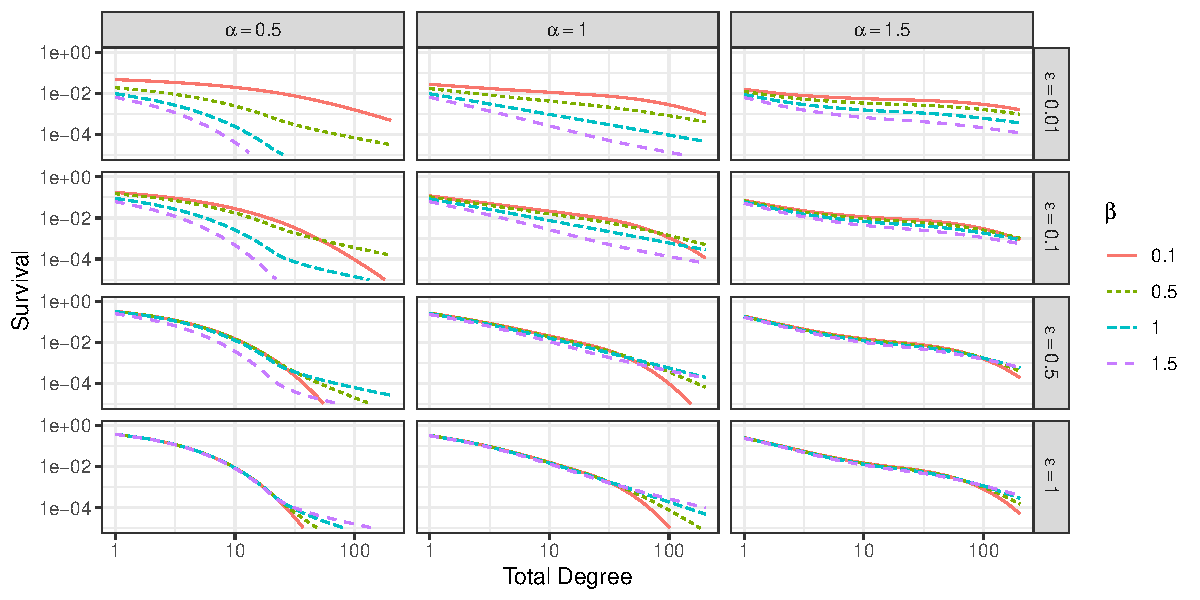
\includegraphics[width=0.8\textwidth,height=\textheight]{paper_files/figure-pdf/fig-polylinsurv-1.pdf}

}

\caption{\label{fig-polylinsurv}Theoretical survival distributions of
the limiting degree distributions, according to various combinations of
\((\alpha, \beta, \varepsilon)\) and \(k_0=20\) of the proposed
preferential attachment model.}

\end{figure}%

The survival (Equation~\ref{eq-polysurv}) can be connected to the IGPD
mentioned in Section~\ref{sec-intro} by using Stirling's approximation
of the gamma function to obtain:

\[
\frac{\Gamma(x+y)}{\Gamma(x)}\approx x^{y},
\] and utilising the expression from Equation~\ref{eq-polysurv}:

\begin{align*}
\bar F(k|k\ge k_0) &= \frac{\Gamma\left(\frac{\lambda^* + k_0^\alpha + \varepsilon}{\beta}\right)}{\Gamma\left(\frac{k_0^\alpha + \varepsilon}{\beta}\right)}\times\frac{\Gamma\left(k-k_0  +1 + \frac{k_0^\alpha + \varepsilon}{\beta}\right)}{\Gamma\left(k-k_0  +1 + \frac{\lambda^*+ k_0^\alpha + \varepsilon}{\beta}\right)}\\
&\approx\left(\frac{k_0^\alpha+\varepsilon}{\beta}\right)^{\lambda^*/\beta}\left(k-k_0+1+\frac{k_0^\alpha + \varepsilon}{\beta}\right)^{-\lambda^*/\beta}\\
&=\left(\frac{k_0^\alpha+\varepsilon}{k_0^\alpha+\varepsilon + \beta}\right)^{\lambda^*/\beta}\left(\frac{\beta(k-k_0)}{\beta + k_0^\alpha+\varepsilon} + 1\right)^{-\lambda^*/\beta}\\
&=\left(\frac{\beta(k+1-k_0)}{k_0^{\alpha}+\varepsilon} + 1\right)^{-\lambda^{*}/\beta}
\end{align*}

\[
\bar F(k) 
\begin{cases}
=\prod_{i=0}^{k}\frac{i^\alpha + \varepsilon}{\lambda^*+i^\alpha + \varepsilon},&k<k_0,\\
\approx \left(\prod_{i=0}^{k_0-1}\frac{i^\alpha + \varepsilon}{\lambda^*+i^\alpha + \varepsilon}\right) \left(\frac{\beta(k+1-k_0)}{k_0^{\alpha}+\varepsilon} + 1\right)^{-\lambda^*/\beta},&k\ge k_0,
\end{cases}
\] meaning that for \(k\ge k_0\) the limiting degree distribution is
similar to
\(\text{IGPD}\left(\frac{\beta}{\lambda^*}, \frac{k_0^\alpha + \varepsilon}{\lambda^*},k_0-1\right)\).

To assess how close of an approximation this is the theoretical
conditional survivals are shown in Figure~\ref{fig-approx_surv} in
colour and their IGPD approximations are shown in grey. The
approximation seems to hold up fairly well even for large degrees.

\begin{figure}[H]

\centering{

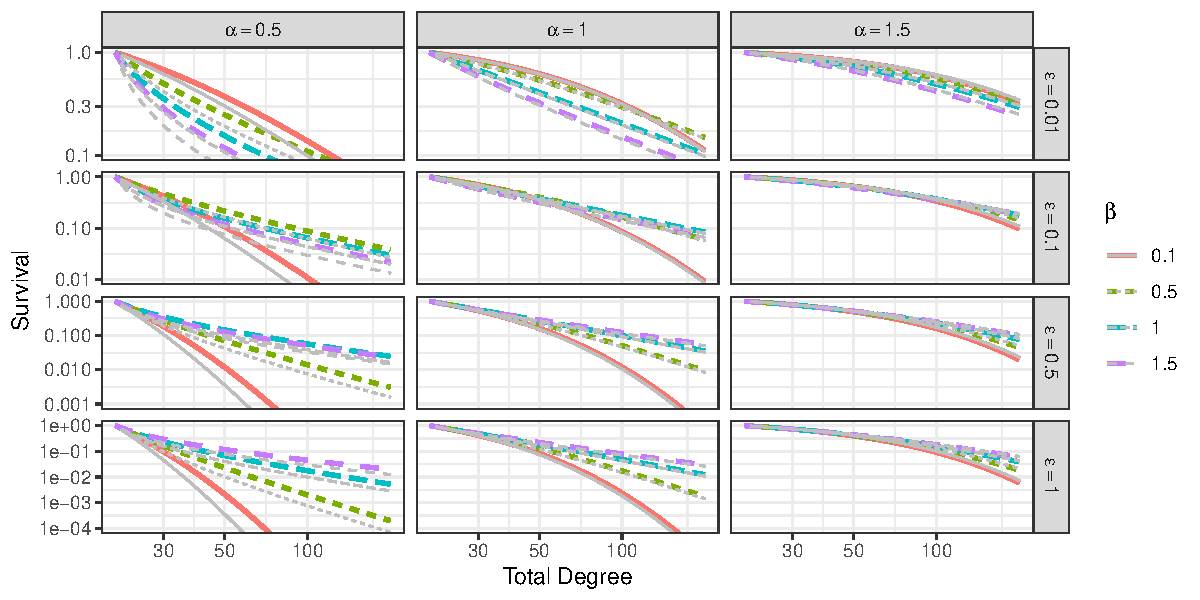
\includegraphics[width=0.8\textwidth,height=\textheight]{paper_files/figure-pdf/fig-approx_surv-1.pdf}

}

\caption{\label{fig-approx_surv}Theoretical conditional survivals (grey)
alongside their IGPD approximations (coloured).}

\end{figure}%

Since \(\beta>0\), the shape parameter of the IGPD is positive and thus
the distribution is heavy tailed. Additionally the value of the shape
parameter \(\xi\) is shown in Figure~\ref{fig-polyheat} for various
parameter choices:

\begin{figure}[H]

\centering{

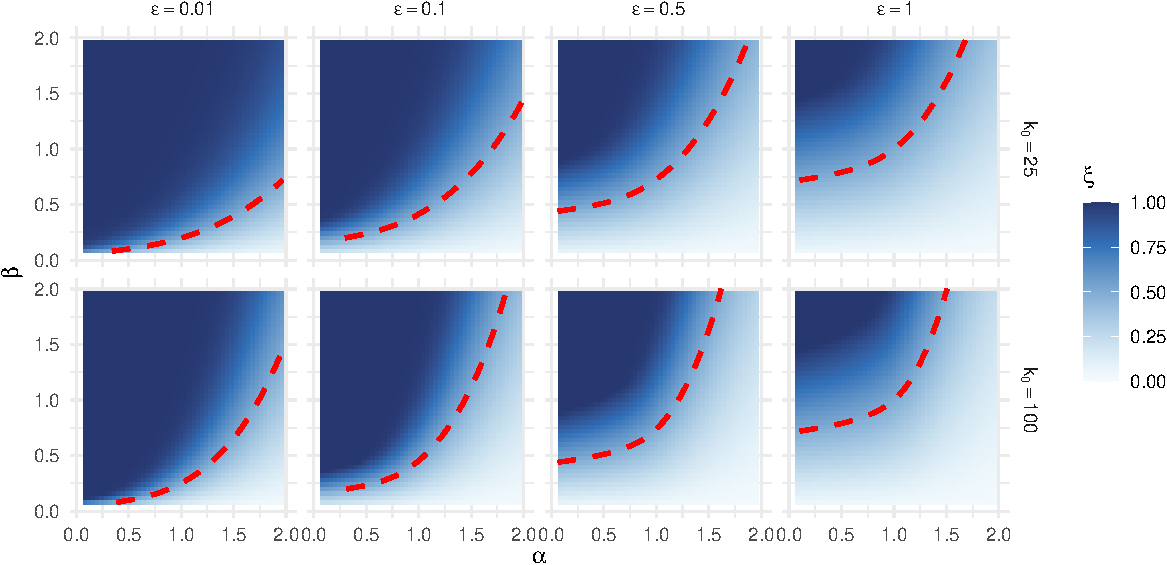
\includegraphics[width=0.8\textwidth,height=\textheight]{paper_files/figure-pdf/fig-polyheat-1.pdf}

}

\caption{\label{fig-polyheat}Heat maps of \(\xi\) for various
combinations of the parameters of the proposed model.}

\end{figure}%

The darker regions on the heat maps correspond to a heavier tail and the
lighter to a lighter tail, the red dashed line shows combinations of
\(\alpha\) and \(\beta\) that produce a limiting degree distribution
with the same tail heaviness as the Barabási-Albert model, \(\xi=0.5\).

For a given network with degree count vector
\(\pmb n = (n_0, n_1, \ldots, n_M)\) and maximum degree \(M\) the
likelihood is given by:

\begin{align*}
L(\pmb x,\pmb n | \pmb \theta) = \left(\frac{\lambda^*}{\lambda^*+\varepsilon}\right)^{n_0}\left(\prod_{j=l}^{k_0-1}\frac{j^\alpha +\varepsilon}{\lambda^* + j^\alpha +\varepsilon}\right)^{\left(\sum_{i\ge k_0}n_{i}\right)} \prod_{l \le i<k_0}\left(\frac{\lambda^*}{\lambda^* +i^\alpha + \varepsilon } \prod_{j=l}^{k_0-1}\frac{j^\alpha + \varepsilon}{\lambda^* + j^\alpha + \varepsilon}\right)^{n_i}\\ \times \prod_{i\ge k_0}\left(\frac{\text{B}(i-k_0 + (k_0^\alpha + \varepsilon)/\beta,1+\lambda^*/\beta)}{\text{B}((k_0^\alpha + \varepsilon)/\beta,\lambda^*/\beta)}\right)^{n_i}
\end{align*}

where \(B(y,z)\) is the the beta function and \(l\ge0\) variable that
allows truncating the data such that the minimum degree is \(l\).

This likelihood allows for the parameters to be inferred using either a
frequentist or a Bayesian approach.

\section{Recovery}\label{sec-rec}

The goal of was to provide a possible preference function that is able
to explain the growth of real networks with varied tail behaviour in
their degree distributions. This section aims to show that the
parameters of the model in Section~\ref{sec-model} can be recovered from
the degree distribution of a network simulated from it.

The procedure for recovering the parameters begins with simulating a
network from the model with \(N=100,000\) vertices and \(m=1\) given
some set of parameters
\(\pmb\theta = (\alpha, \beta, \varepsilon, k_0)\), obtaining the degree
counts in the form of a vector of degrees \(\pmb x = (1,2,\ldots,M)\)
and the number of vertices with those degrees \(\pmb n\) where \(M\) is
the maximum degree. However, when it comes to fitting this model to real
data in the next section, small degrees are extremely influential and
will often cause the model to have a bad fit even though the rest of the
data looks similar to that of the simulations; truncating the data above
some value, say \(l<k_0\), should allow the model to be more effectively
fitted. This accounts in some way for the fact that this model only
applies to trees, and could not possibly capture the behaviour for nodes
with small degrees. Using the p.m.f derived in \citep{rudas07}, the
likelihood given that \(x_i \ge l\) for all \(i =1,2,\ldots,M\) is:

\begin{align*}
L(\pmb x,\pmb n | \pmb \theta) = \left(\frac{\lambda^*}{\lambda^*+\varepsilon}\right)^{n_0}\left(\prod_{j=l}^{k_0-1}\frac{j^\alpha +\varepsilon}{\lambda^* + j^\alpha +\varepsilon}\right)^{\left(\sum_{x_i\ge k_0}n_{x_i}\right)} \prod_{l \le x_i<k_0}\left(\frac{\lambda^*}{\lambda^* +x_i^\alpha + \varepsilon } \prod_{j=l}^{k_0-1}\frac{j^\alpha + \varepsilon}{\lambda^* + j^\alpha + \varepsilon}\right)^{n_i}\\ \times \prod_{x_i\ge k_0}\left(\frac{\text{B}(x_i-k_0 + (k_0^\alpha + \varepsilon)/\beta,1+\lambda^*/\beta)}{\text{B}((k_0^\alpha + \varepsilon)/\beta,\lambda^*/\beta)}\right)^{n_i}
\end{align*}

where \(B(y,z)\) is the the beta function.

This likelihood allows inference to be made about the parameters using a
Bayesian approach using the priors:

\begin{align*}
\alpha&\sim \text{Ga}(1,0.01),\\
\beta &\sim  \text{Ga}(1,0.01),\\
k_0 &\sim \text{U}(1,10,000),\\
\varepsilon &\sim \text{Ga(1,0.01)},
\end{align*}

to obtain a posterior distribution that can then be used in an adaptive
Metropolis-Hastings Markov chain Monte Carlo (MCMC) algorithm to obtain
posterior samples. The results of this inference are shown in
Figure~\ref{fig-rec1} and Figure~\ref{fig-rec2}. For these simulated
networks \(l=0\).

\begin{figure}[H]

\centering{

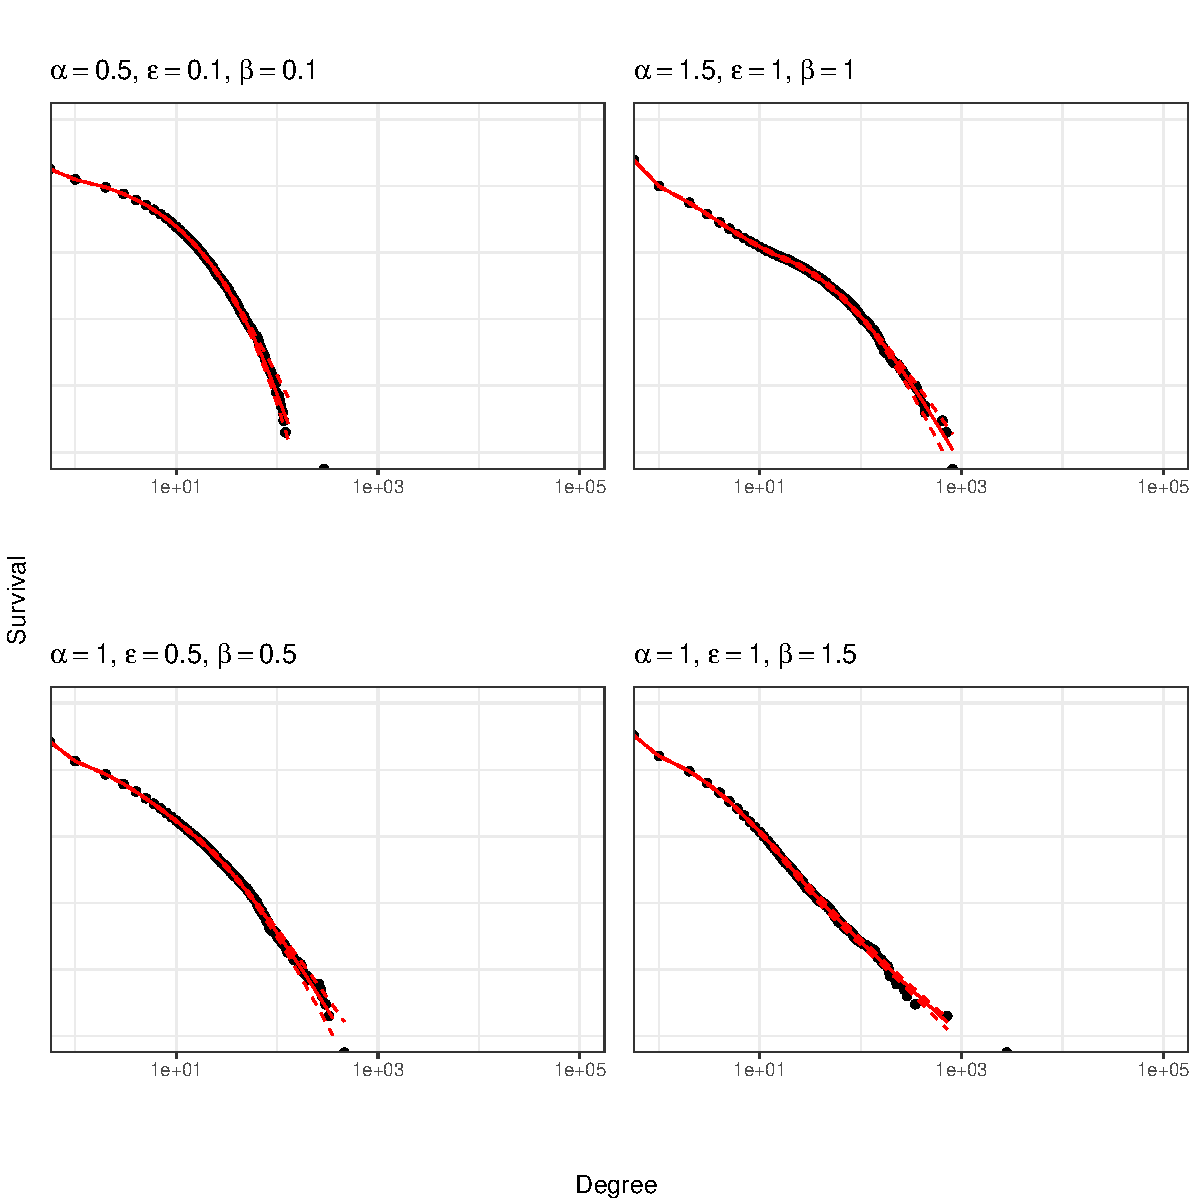
\includegraphics[width=0.8\textwidth,height=\textheight]{paper_files/figure-pdf/fig-rec1-1.pdf}

}

\caption{\label{fig-rec1}Posterior estimates of survival function for
data simulated from the proposed model with various combinations of
(\(\alpha\),\(\beta\),\(\varepsilon\)) and \(k_0=20\).}

\end{figure}%

\begin{figure}[H]

\centering{

\captionsetup{labelsep=none}

\begin{figure}[H]

{\centering 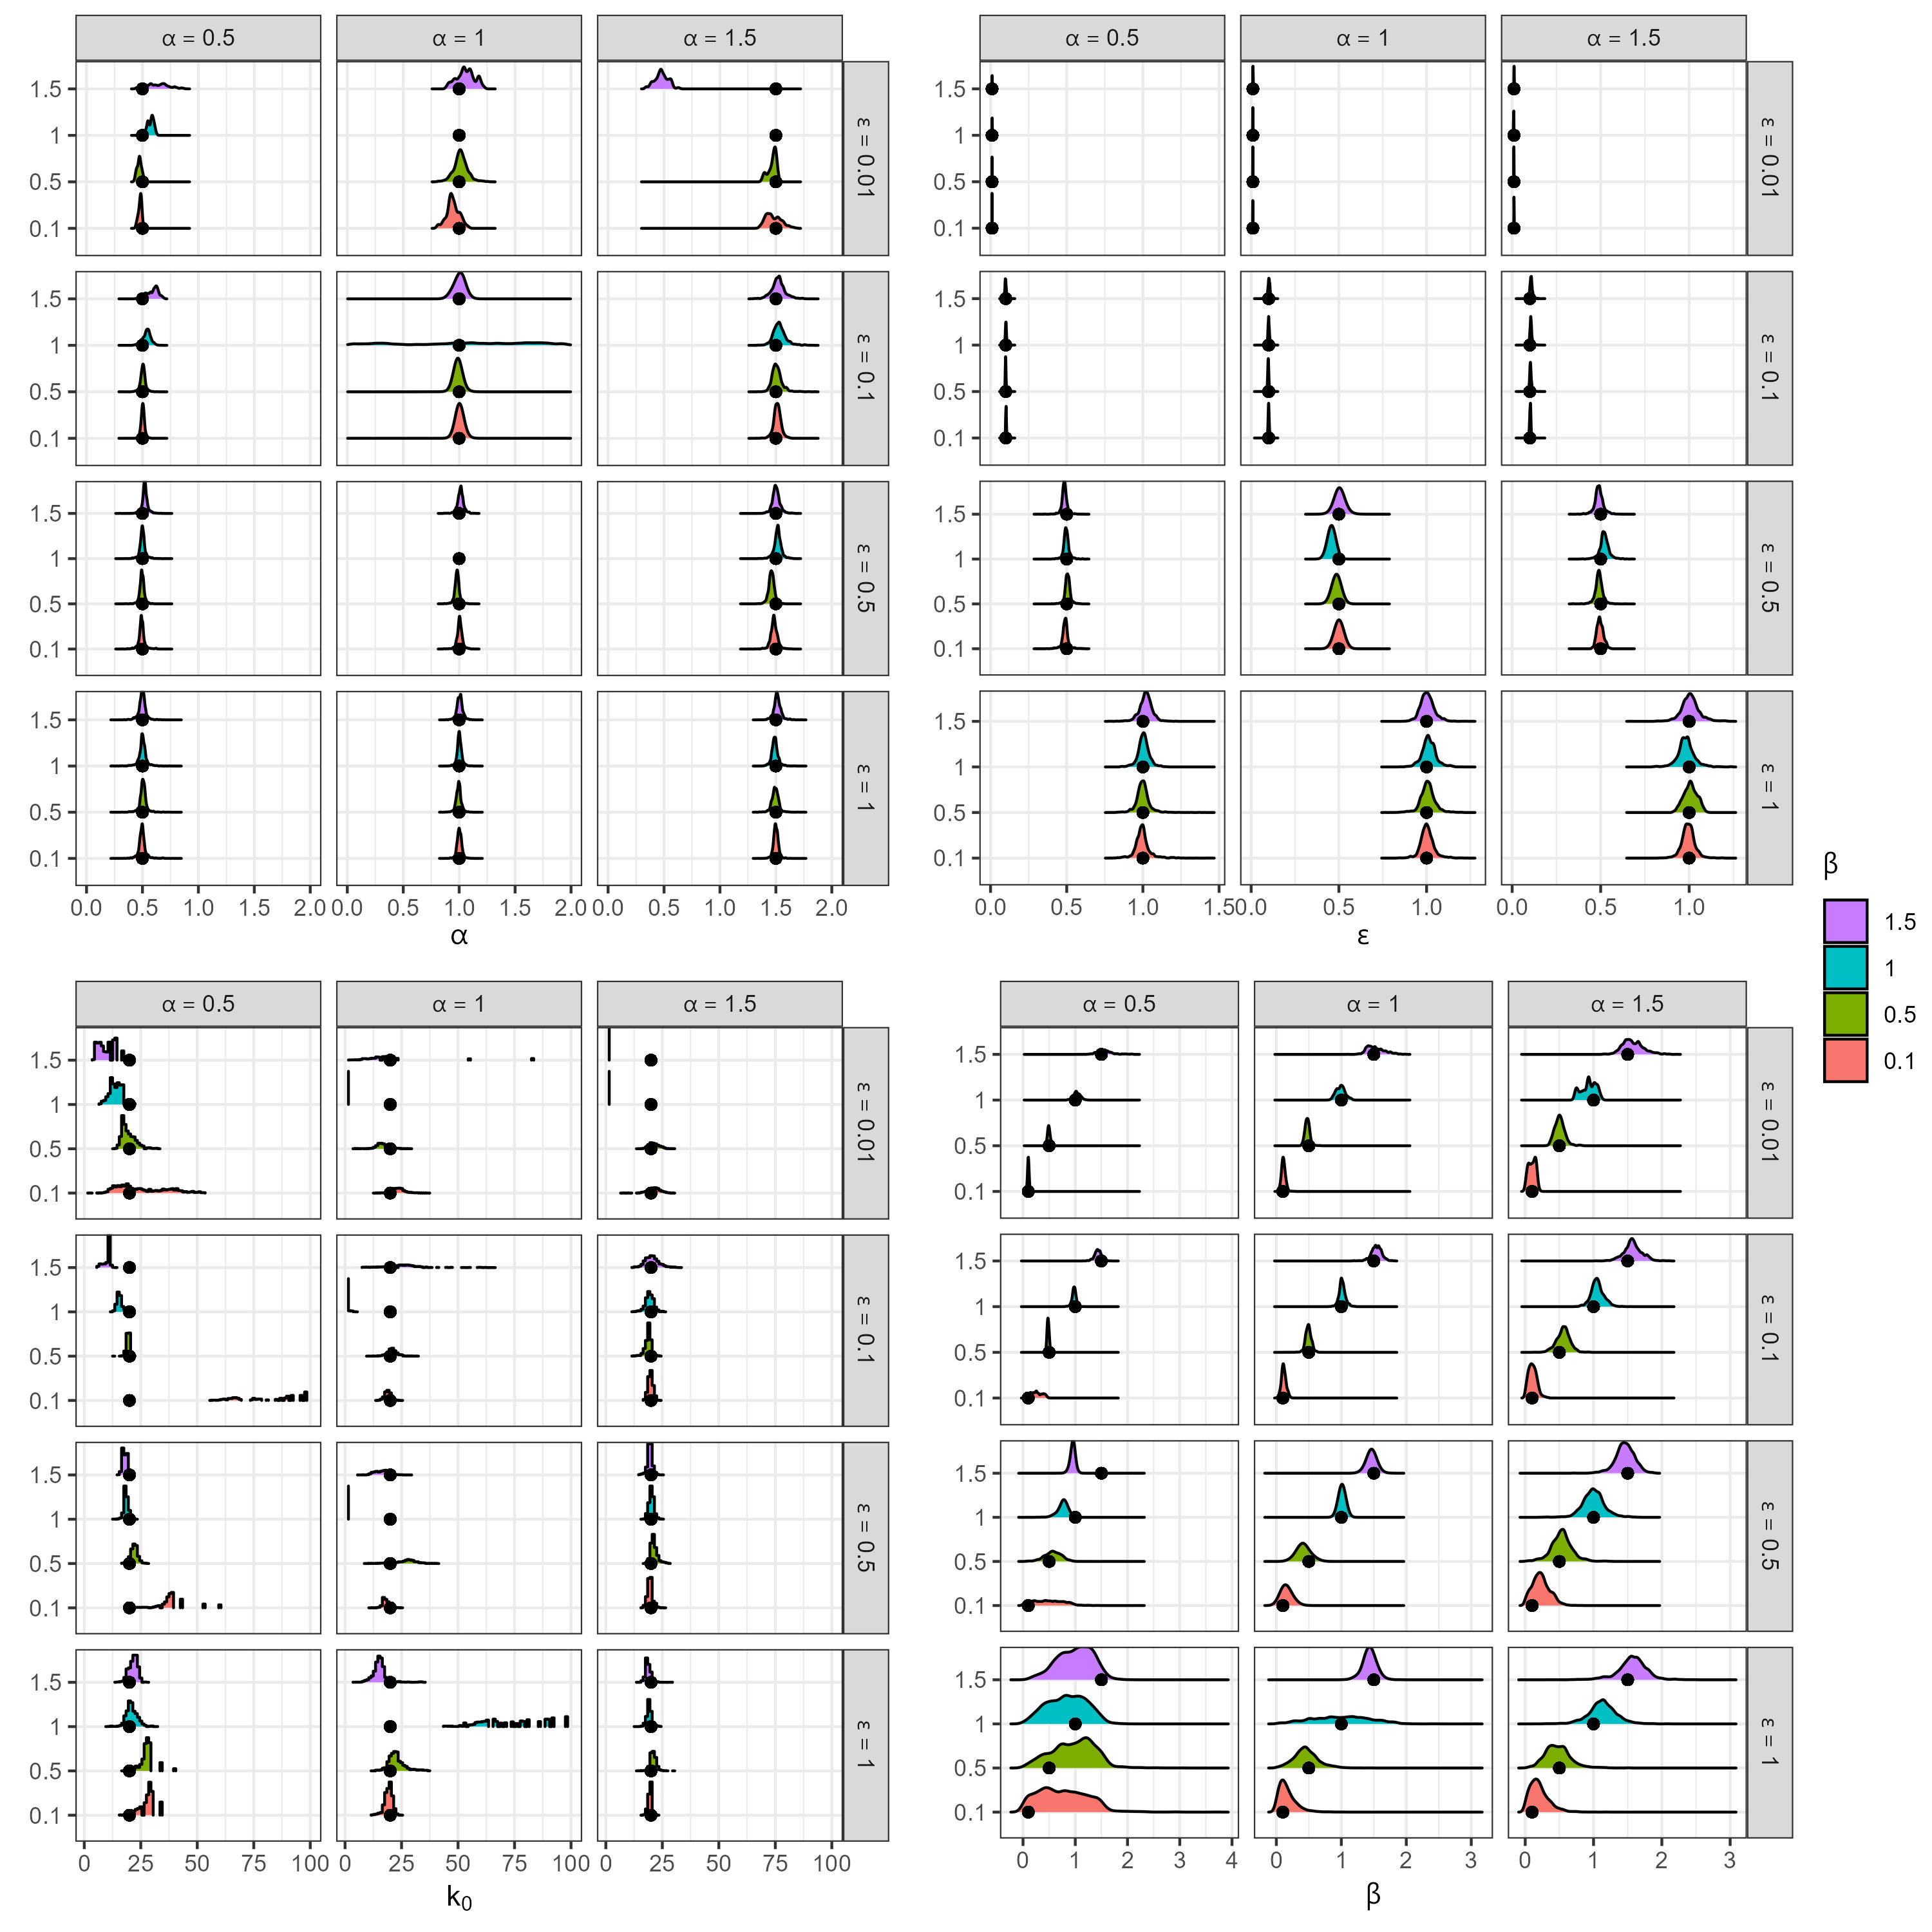
\includegraphics{mcmc_plot.jpg}

}

\caption{: Posterior estimates of paramters for data simulated from the
proposed model with various combinations of
(\(\alpha\),\(\beta\),\(\varepsilon\)) and \(k_0=20\).}

\end{figure}%

}

\caption{\label{fig-rec2}}

\end{figure}%

Figure~\ref{fig-rec1} and Figure~\ref{fig-rec2} demonstrate that using
this methodology it is possible to recover the model parameters fairly
well from only the final degree distribution of a simulated network.
This indicates that the method may also be able to be applied to the
degree distributions of real networks, estimating the model parameters
assuming they evolved according to the GPA scheme.

\section{Application to Real Data}\label{sec-real}

Turning now to real data, the goal is to fit the model to the degree
distributions of real networks from various sources. {[}describe
networks being used{]}. Alongside fitting this model to the degree
distributions, we then compare the fit to that of an mixture
distribution that was used in {[}clement{]} and is similar to others
that have been used to model degree distributions {[}others{]}.

\begin{figure}[H]

\centering{

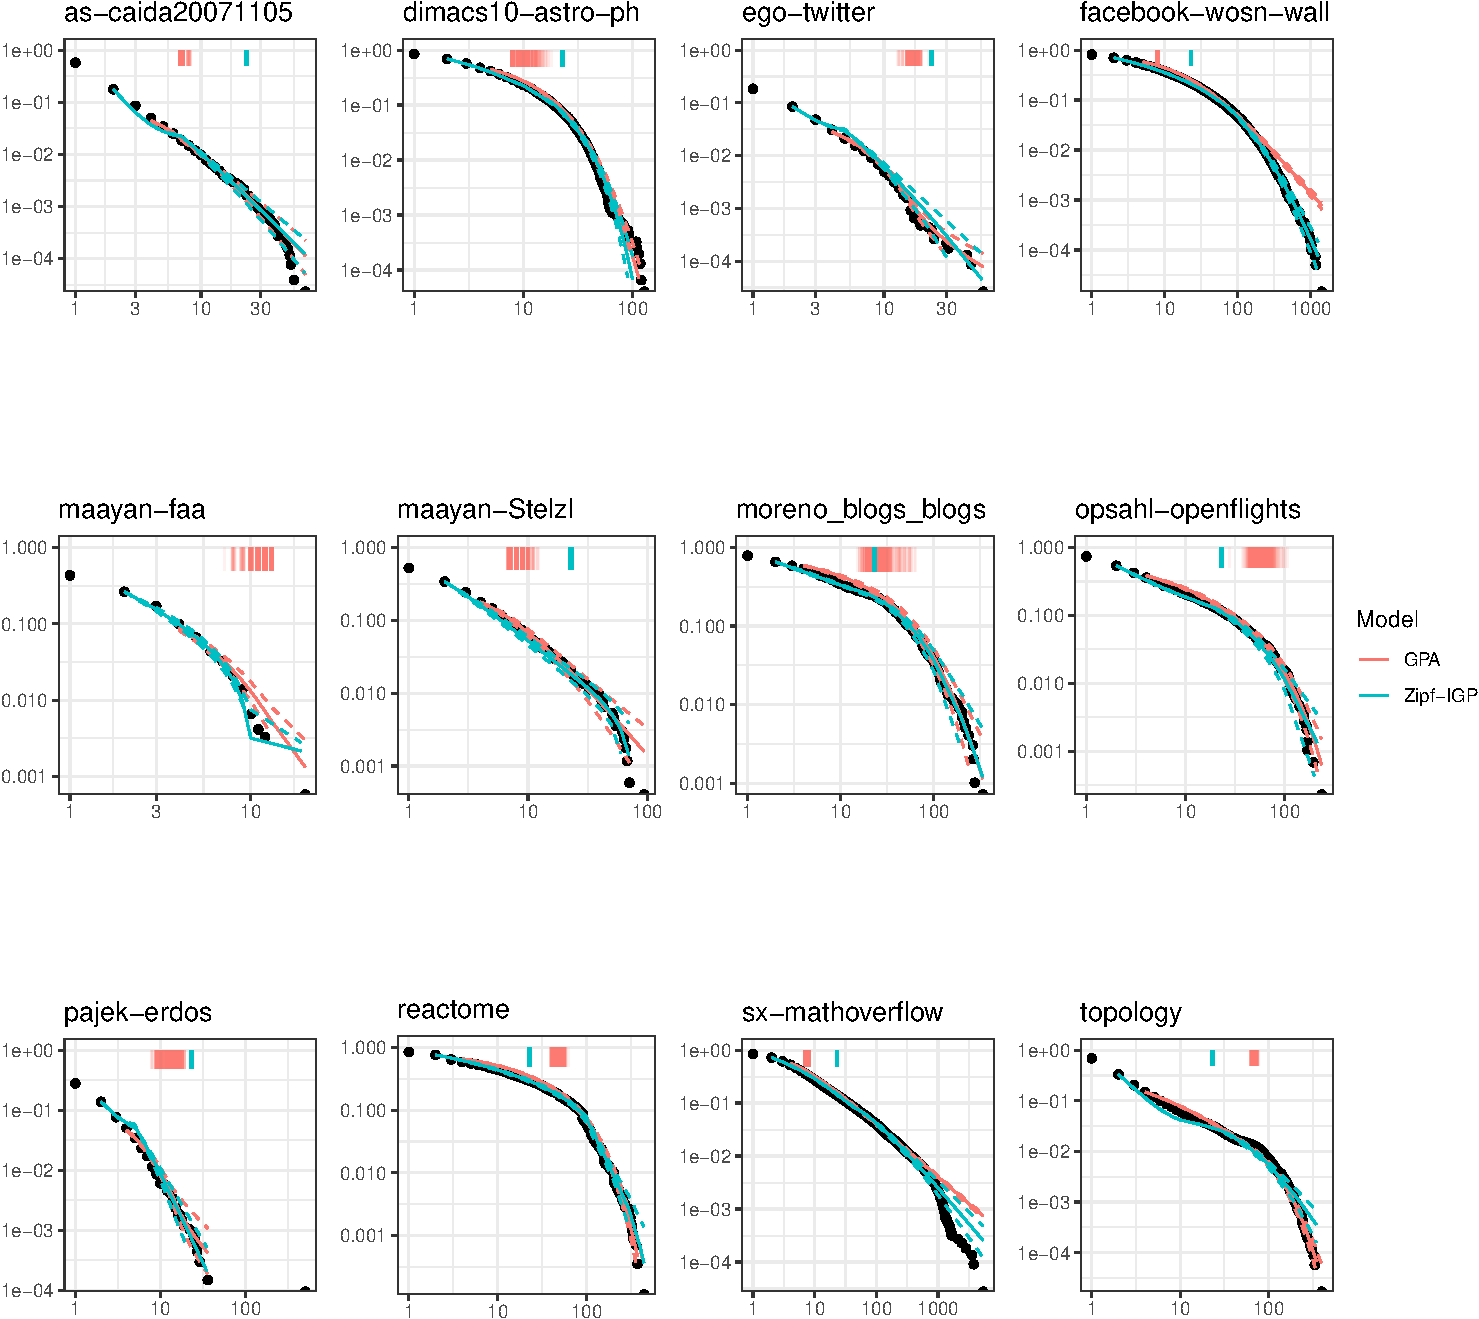
\includegraphics[width=0.8\textwidth,height=\textheight]{paper_files/figure-pdf/fig-real1-1.pdf}

}

\caption{\label{fig-real1}Posterior estimates (solid red) of survival
for several real data sets and their 95\% credible intervals (dotted
red)}

\end{figure}%

Figure~\ref{fig-real1} displays the posterior estimates of the survival
function for various data sets, obtained from fitting the GPA model and
the Zipf-IGP mixture model. In most cases, the GPA model does not
necessarily provide an improvement in fit when compared to the Zipf-IGP
model but where the GPA model fits well we gain additional information
about the preference function assuming that the network evolved
according the the GPA scheme. Figure~\ref{fig-shapes} shows the
posterior of the shape parameter \(\xi\) obtained from the Zipf-IGP
model alongside the posterior of the equivalent shape parameter
\(\beta/\lambda^*\) obtained from fitting the GPA model. Generally, the
GPA model performs similarly to the Zipf-IGP when estimating the tail
behaviour of the degree distribution and where it doesn't it appears to
either be because it is fitting better at the tail than the Zipf-IGP
model or because of the threshold being estimated as too low forcing
almost all of the data to be modelled by the linear part of the GPA.
This again shows the effects that small degrees have on this model,
which is somewhat expected as the theory used for this model is for
trees and none of these real networks (nor many real networks) are.

\begin{figure}[H]

\centering{

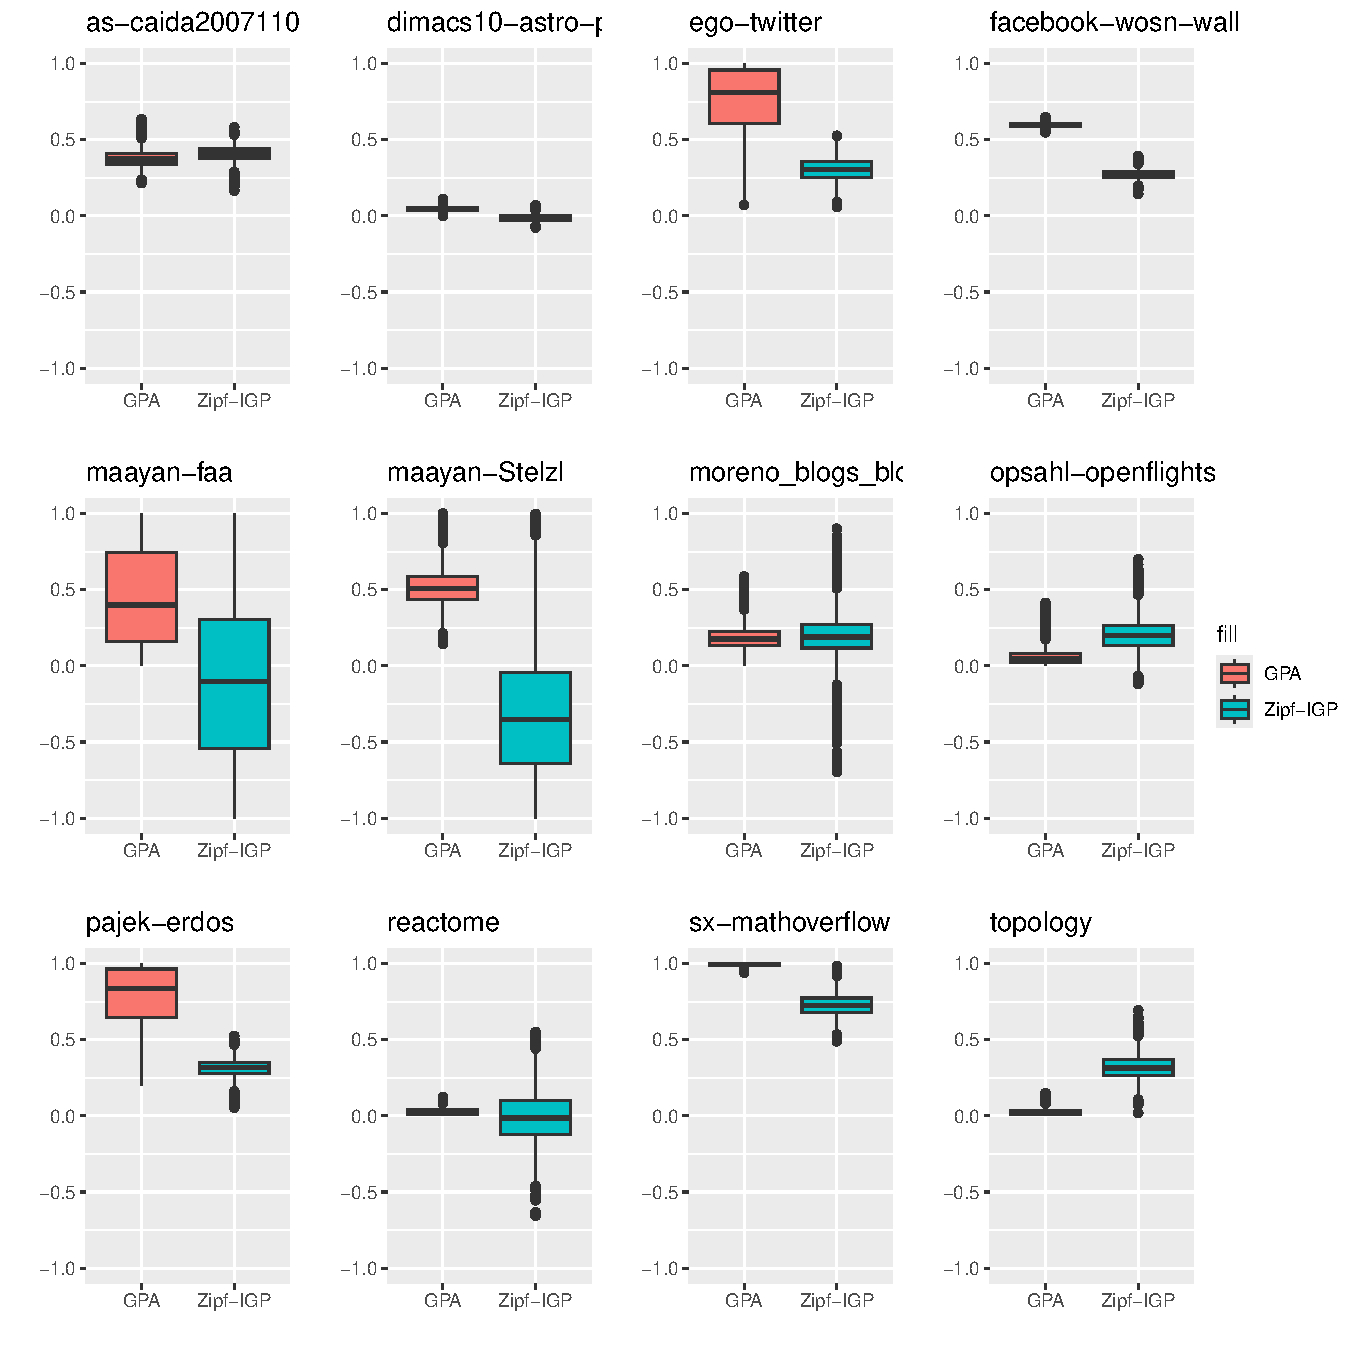
\includegraphics[width=0.8\textwidth,height=\textheight]{paper_files/figure-pdf/fig-shapes-1.pdf}

}

\caption{\label{fig-shapes}Posterior estimates (solid red) of survival
for several real data sets and their 95\% credible intervals (dotted
red)}

\end{figure}%

Figure~\ref{fig-pa} shows the estimated preference function \(b\)
alongside the 95\% credible interval on a log-log plot. Although the
credible interval becomes very large for the largest degrees, this is
expected as not all of these networks had data in that region, for those
that do the credible interval is much narrower as is the case for
\texttt{sx-mathoverflow}. The most insightful conclusion we can draw
from these plots come from the shape of the preference function. There
appears to be two distinct shapes of preference function. The first
appears mostly flat (similar to UA) for the smallest degrees and then
after a threshold PA kicks in, some with this shape are
\texttt{pajek-erdos} and \texttt{sx-mathoverflow}. The second distinct
shape appears provide some clear PA behaviour that then slows down after
a certain point, examples of this are seen in the two infrastructure
networks \texttt{opsahl-openflights} and \texttt{topology}.

\begin{figure}[H]

\centering{

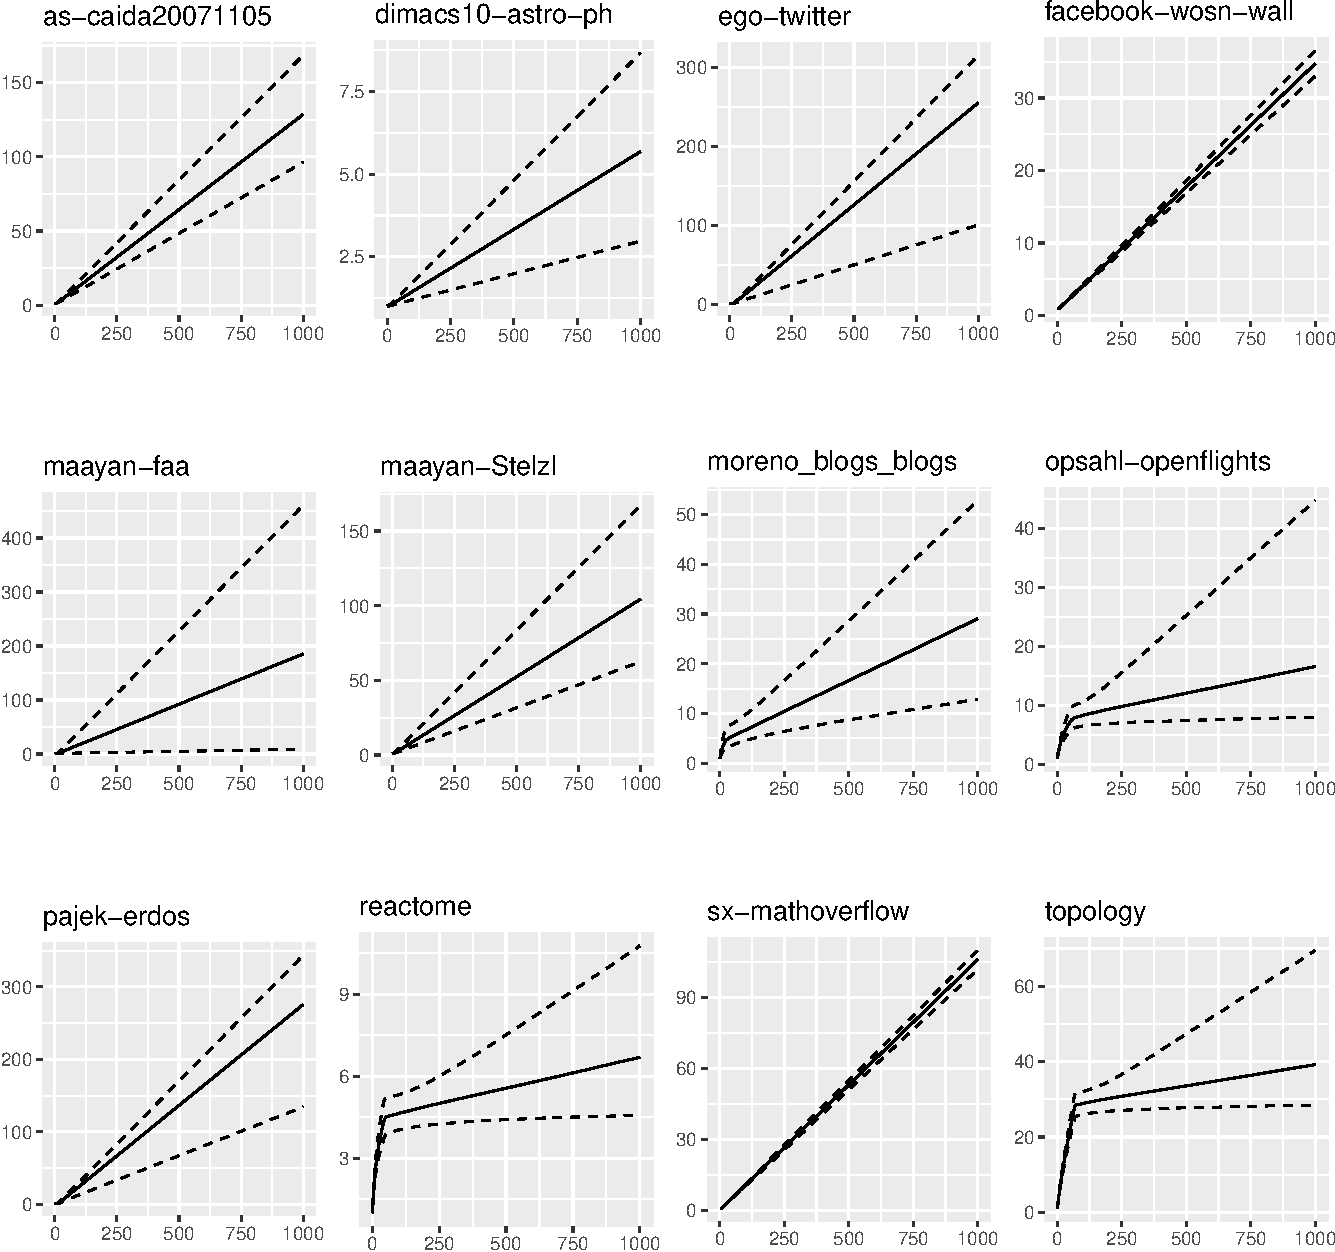
\includegraphics[width=0.8\textwidth,height=\textheight]{paper_files/figure-pdf/fig-pa-1.pdf}

}

\caption{\label{fig-pa}Posterior estimate for preference function
(solid) with 95\% credible interval (dashed) on log-log scale.}

\end{figure}%

\begin{figure}[H]

\centering{

\captionsetup{labelsep=none}

\begin{figure}[H]

{\centering 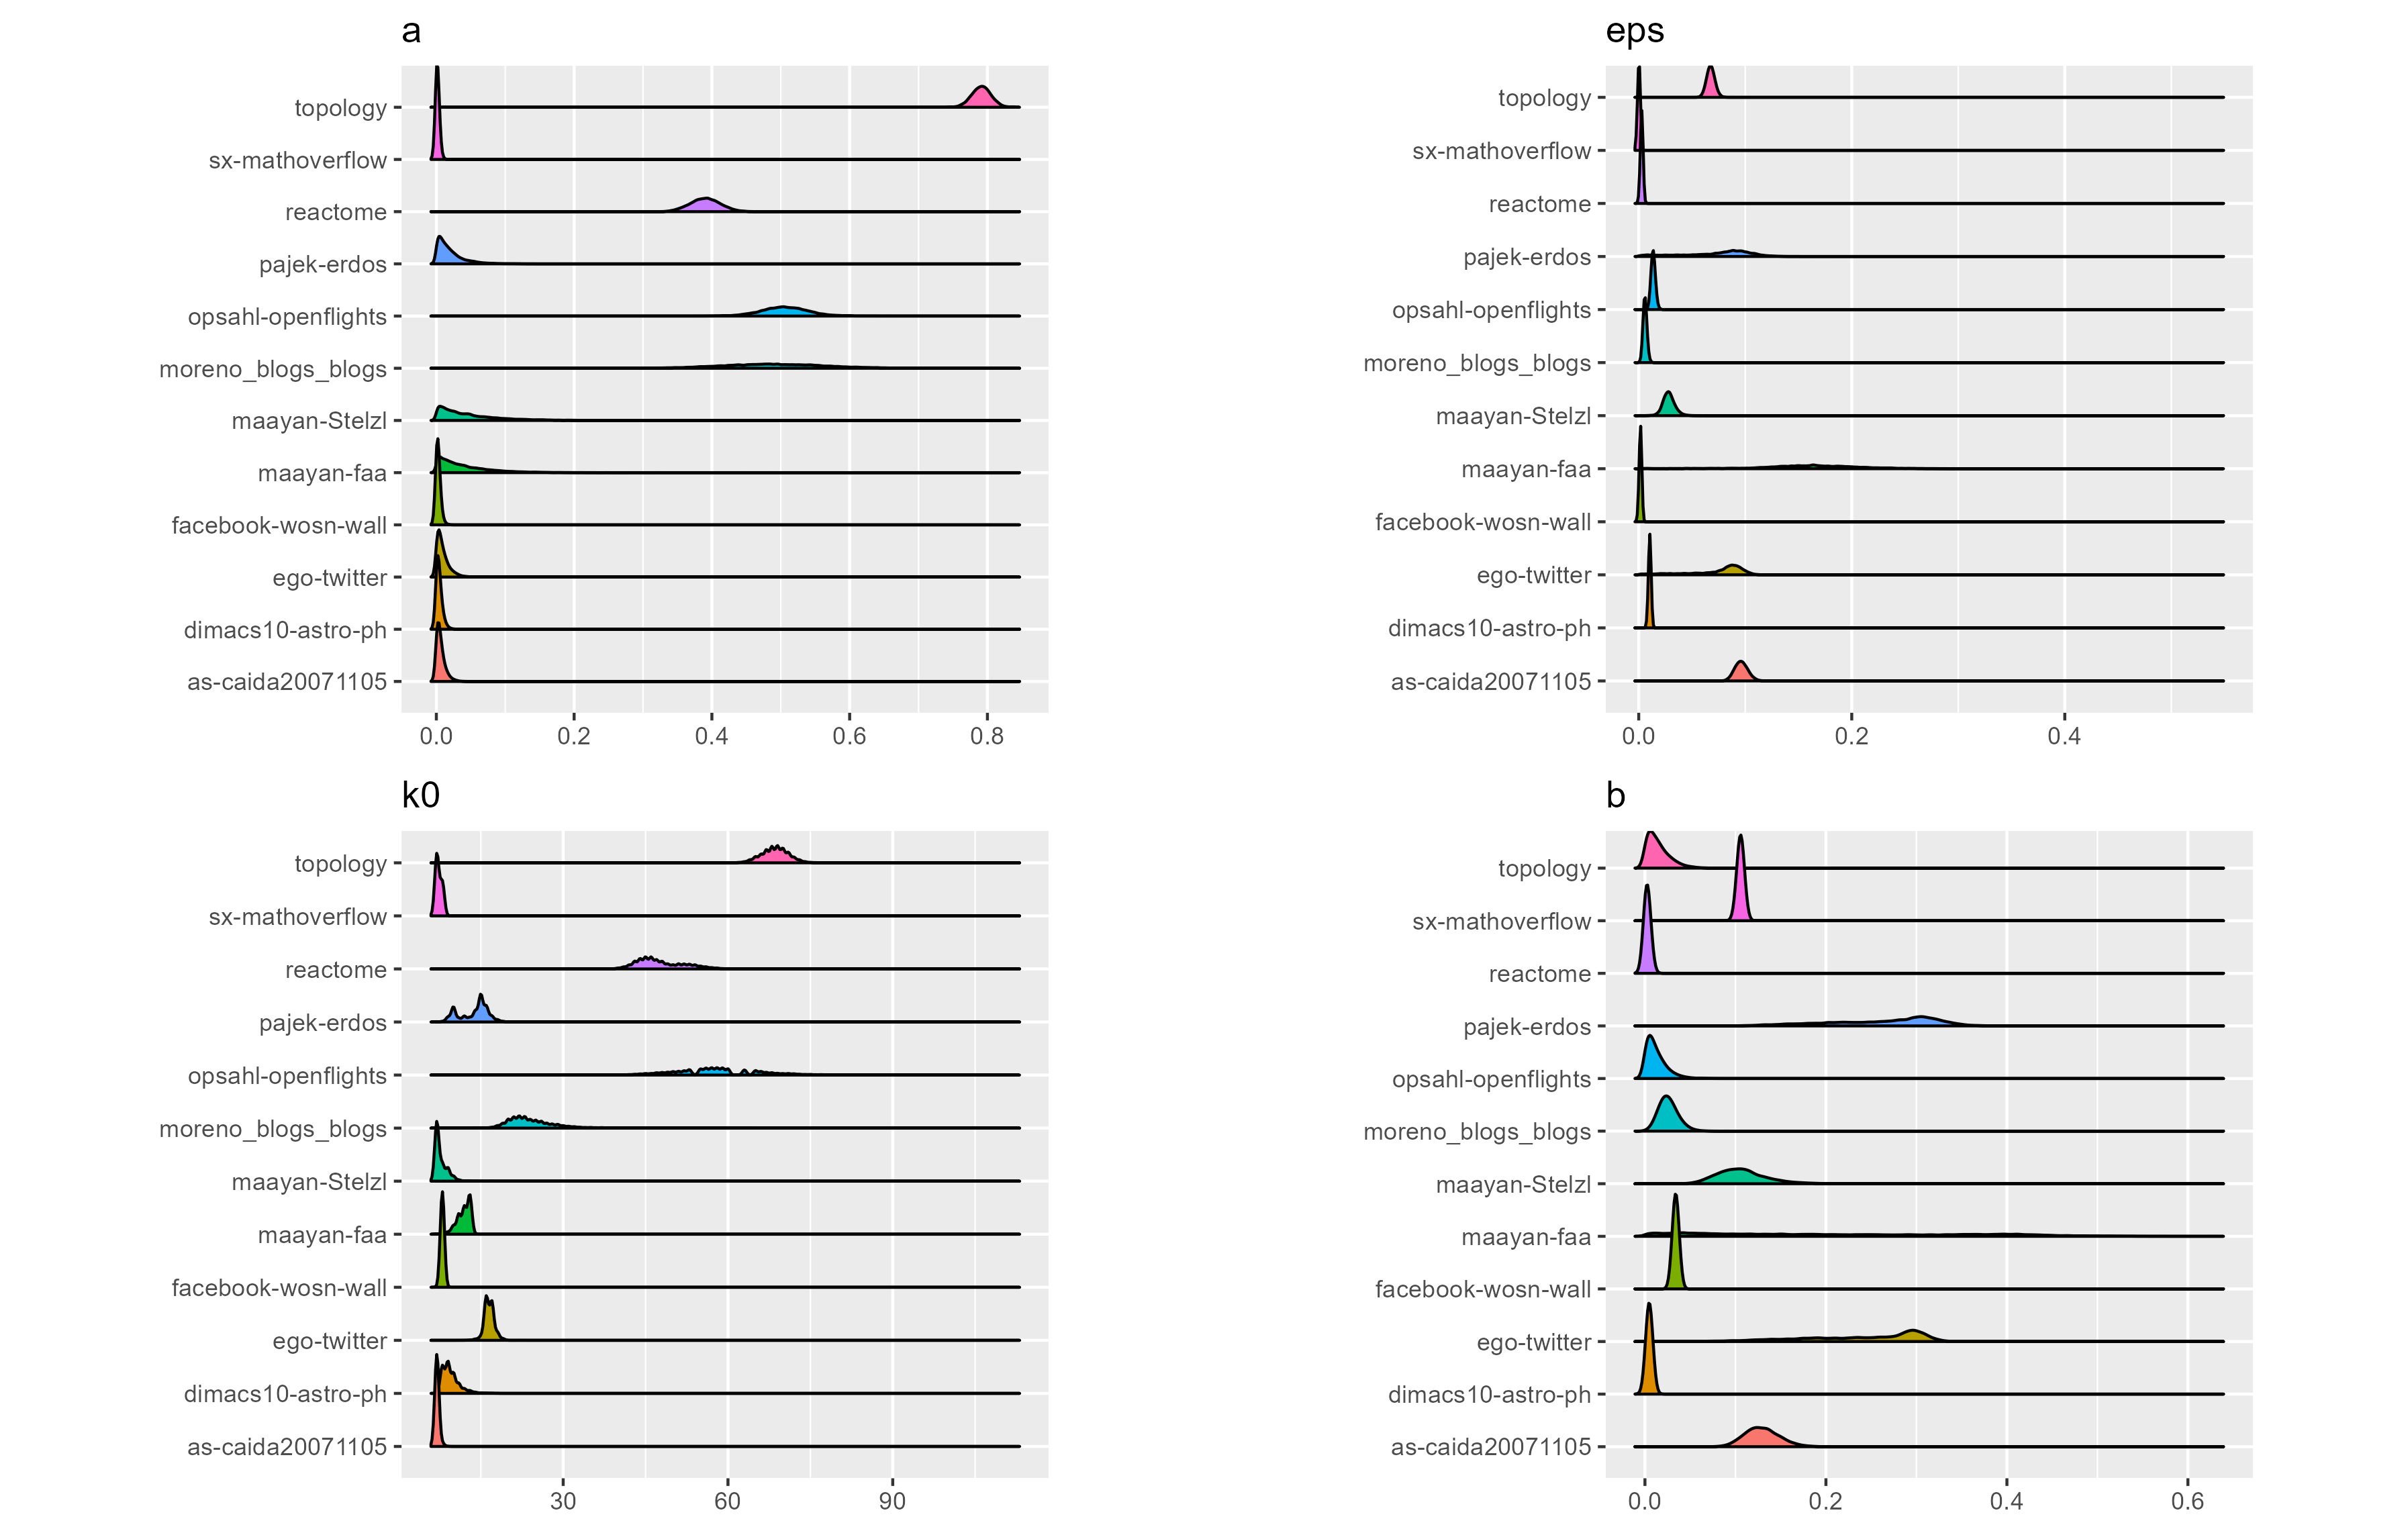
\includegraphics{pars_plot.png}

}

\caption{: Posterior estimates of paramters for real data.}

\end{figure}%

}

\caption{\label{fig-rec2}}

\end{figure}%

\section{Conclusion and Discussion}\label{sec-conc}

In this paper we introduced a flexible class of preference function that
when used under the GPA scheme (in the tree setting) is guaranteed to
generate a network with a heavy tailed degree distribution whilst
remaining flexible in the body. Using simulations from networks using
this class of preference function we showed that the model parameters
are quite easily estimated from the degrees alone at a snapshot in time.
Seeing this we applied this method to the degree distributions of real
networks, estimating their model parameters assuming they evolved in the
same way. Not only did this yield fairly good fits for the degree
distribution, similar to that of the Zipf-IGP, it came with the added
benefit of giving a posterior estimate for a preference function.

Obviously this method had its flaws in that the lowest degrees needed to
be truncated as they had a very large effect on the fit of the model as
a result of using theory developed for trees and applying it to general
networks. Hopefully, as the field progresses we will be able to apply
theory developed for general networks using a similar method to this,
allowing us to compare the results here something that is more accurate.

GPA is also a fairly simplistic one on its own despite having large
flexibility in the preference function allowing for edges to only be
added at times when a new node is introduced into the network and not
allowing for anything like vertex/edge death, reciprocal edges and
rewiring steps. \citep{deijfen2015} introduces some theory for GPA with
vertex death based on the work by \citep{rudas07}, but is unable to come
to an expression for the degree distribution. However, adding something
like fitness scores into the GPA model seems fairly simple to do even
going so far as making each of the parameters used in the class of
functions here node-wise instead of universal. For example having the
preference weight for a vertex be given by
\(b(k_i, \underline{\gamma_i})\) where \(\underline{\gamma_i}\sim G\) is
the vertex's fitness and \(k_i\) is the vertex's degree, it is
reasonable to expect that the degree distribution for a model like this
to be given by:

\[
\bar F(k) = \mathbb E_G\left[\prod_{i=0}^k \frac{b(i, \gamma)}{\lambda^* + b(i,\gamma)}\right],\qquad \gamma\sim G,\, k=0,1,2,\ldots
\]

If this were the case, the posterior distributions of parameters from
Section~\ref{sec-real} could be interpreted as the approximate
distributions from which a vertex's fitness values are drawn instead of
providing estimates of the universal parameter values. Additionally, it
allows the ability to set some parameters as universal and some as
vertex-wise for example one could let \(\alpha, \beta, k_0\) be the same
for all vertices but let each vertex in the network have its own ``zero
appeal''
\(\varepsilon_i\overset{\text{iid}}{\sim} \text{Ga}(\theta_1, \theta_2)\);
moving the model to being more realistic and accounting for the fact
that in many real networks the objects vertices represent have some
value instrinsic to themselves other than the number of connections they
have.

\section{Appendix}\label{appendix}

\subsection{Additional Results}\label{additional-results}

\subsubsection{Tail heaviness of general preferential attachment
model}\label{tail-heaviness-of-general-preferential-attachment-model}

Recall the limiting survival function:

\[
\bar F(k) = \prod_{i=0}^k \frac{b(i)}{\lambda^*+b(i)},
\]

The aim is to determine how this distribution behaves for different
choices of \(b\), specifically what maximum domain of attraction does
this distribution belong to and is it affected by the choice of
preference function \(b\). \citet{shimura12} introduces a quantity that
will help in determining what domain of attraction a discrete
distribution belongs to, that is:

For a distribution \(F\) with survival function \(\bar F\) and some
\(n\in\mathbb Z^+\) let:

\[
\Omega(F,n) = \left(\log\displaystyle\frac{\bar F (n+1)}{\bar F (n+2)}\right)^{-1} - \left(\log\displaystyle\frac{\bar F (n)}{\bar F (n+1)}\right)^{-1}
\]

\citep{shimura12} then states that if
\(\lim_{n\rightarrow\infty} \Omega(F,n) = 1/\alpha\) (\(\alpha>0\)),
then \(F\) is heavy tailed with \(\bar F(n) \sim n^{-\alpha}\).
Additionally, if \(\lim_{n\rightarrow\infty} \Omega(F,n) = 0\) then the
distribution is light tailed.

Consider a preference function \(b(\cdot)\) that fulfills:

\begin{equation}\phantomsection\label{eq-condb1}{
\lim_{n\rightarrow \infty} b(n) = \infty
}\end{equation}

Substituting in the form of \(\bar F(n)\) from \textbf{?@eq-surv} and
taking the limit, subject to Equation~\ref{eq-condb1}:

\begin{equation}\phantomsection\label{eq-omegares}{
\lim_{n\rightarrow\infty}\Omega(F,n) = \lim_{n\rightarrow\infty}\frac{b(n+2)-b(n+1)}{\lambda^*}.
}\end{equation} (see appendix for full proof).

Whilst there are many classes of functions that satisfy
Equation~\ref{eq-condb1} and Equation~\ref{eq-condb2}, the vast majority
of these result in \(\Omega(F,n) \rightarrow 0\), meaning that the
limiting degree distribution is light tailed. In fact, in order for the
limiting degree distribution to be heavy tailed, \(b\) must be
asymptotically linear (\(b(k)\sim k\)).

\subsection{Proofs}\label{proofs}

\subsubsection{Tail heaviness of GPA}\label{tail-heaviness-of-gpa}

Taking the form of the GPA degree survival: \[
\bar F(n) = \prod_{i=0}^n\frac{b(i)}{\lambda+b(i)}
\] and substituting into the formula for \(\Omega(F,n)\):

\begin{align*}
\Omega(F,n)&=\left(\log\frac{\prod_{i=0}^{n+1}\frac{b(i)}{\lambda+b(i)}}{\prod_{i=0}^{n+2}\frac{b(i)}{\lambda+b(i)}}\right)^{-1}-\left(\log\frac{\prod_{i=0}^{n}\frac{b(i)}{\lambda+b(i)}}{\prod_{i=0}^{n+1}\frac{b(i)}{\lambda+b(i)}}\right)^{-1}\\
&=\left(\log\frac{\lambda+b(n+2)}{b(n+2)}\right)^{-1}-\left(\log\frac{\lambda+b(n+1)}{b(n+1)}\right)^{-1}\\
&=\left(\log\left[1+\frac{\lambda}{b(n+2)}\right]\right)^{-1}-\left(\log\left[1+\frac{\lambda}{b(n+1)}\right]\right)^{-1}
\end{align*}

Clearly if \(b(n)=c\) or \(\lim_{n\rightarrow\infty}b(n)=c\) for some
\(c>0\) then \(\Omega(F,n)=0\). Now consider a non-constant \(b(n)\) and
re-write \(\Omega(F,n)\) as:

\begin{align*}
\Omega(F,n) &= \left(\log\left[1+\frac{\lambda}{b(n+2)}\right]\right)^{-1}-\frac{b(n+2)}{\lambda}+\frac{b(n+2)}{\lambda}-\left(\log\left[1+\frac{\lambda}{b(n+1)}\right]\right)^{-1}+\frac{b(n+1)}{\lambda}  -\frac{b(n+1)}{\lambda}\\
&=\left\{ \left(\log\left[1+\frac{\lambda}{b(n+2)}\right]\right)^{-1}-\frac{b(n+2)}{\lambda}\right\} - \left\{ \left(\log\left[1+\frac{\lambda}{b(n+1)}\right]\right)^{-1}-\frac{b(n+1)}{\lambda}\right\}+\frac{b(n+2)}{\lambda}-\frac{b(n+1)}{\lambda}
\end{align*}

Then if \(\lim_{n\rightarrow\infty}b(n)=\infty\) it follows that:

\begin{align*}
\lim_{n\rightarrow\infty}\Omega(F,n) &= \lim_{n\rightarrow\infty}\left\{ \left(\log\left[1+\frac{\lambda}{b(n+2)}\right]\right)^{-1}-\frac{b(n+2)}{\lambda}\right\} - \lim_{n\rightarrow\infty}\left\{ \left(\log\left[1+\frac{\lambda}{b(n+1)}\right]\right)^{-1}-\frac{b(n+1)}{\lambda}\right\}\\
&\qquad+\lim_{n\rightarrow\infty}\left(\frac{b(n+2)}{\lambda}-\frac{b(n+1)}{\lambda}\right)\\
&=\frac{1}{2}-\frac{1}{2} + \lim_{n\rightarrow\infty}\left(\frac{b(n+2)}{\lambda}-\frac{b(n+1)}{\lambda}\right)\\
&=\frac{1}{\lambda}\lim_{n\rightarrow\infty}\left[b(n+2)-b(n+1)\right]\qquad \square
\end{align*}

\subsubsection{Removing the infinite
sum}\label{removing-the-infinite-sum}

For a preference function of the form:

\[
b(k) = \begin{cases}
g(k),&k<k_0\\
g(k_0) + \beta(k-k_0), &k\ge k_0
\end{cases}
\] for \(\beta>0, k_0\in\mathbb N\) we have that

\begin{align*}
\hat\rho(\lambda) = \sum_{n=0}^\infty\prod_{i=0}^{n-1}\frac{b(i)}{\lambda+b(i)} &= \sum_{n=0}^{k_0}\prod_{i=0}^{n-1}\frac{g(i)}{\lambda+g(i)} + \sum_{n=k_0+1}^\infty\left(\prod_{i=0}^{k_0-1}\frac{g(i)}{\lambda+g(i)}\prod_{i=k_0}^{n-1}\frac{g(k_0) + \beta(i-k_0)}{\lambda +g(k_0) + \beta(i-k_0)}\right)\\
&=\sum_{n=0}^{k_0}\prod_{i=0}^{n-1}\frac{g(i)}{\lambda+g(i)} + \left(\prod_{i=0}^{k_0-1}\frac{g(i)}{\lambda+g(i)}\right)\sum_{n=k_0+1}^\infty\prod_{i=k_0}^{n-1}\frac{g(k_0) + \beta(i-k_0)}{\lambda +g(k_0) + \beta(i-k_0)}
\end{align*}

Now using the fact that:

\[
\prod_{i=0}^n(x+yi) = x^{n+1}\frac{\Gamma(\frac{x}{y}+n+1)}{\Gamma(\frac{x}{y})}
\] and reindexing the product in the second sum

\begin{align*}
\hat\rho(\lambda) &= \sum_{n=0}^{k_0}\prod_{i=0}^{n-1}\frac{g(i)}{\lambda+g(i)} + \left(\prod_{i=0}^{k_0-1}\frac{g(i)}{\lambda+g(i)}\right)\sum_{n=k_0+1}^\infty\frac{\Gamma\left(\frac{g(k_0)}{\beta}+n-k_0\right)\Gamma\left(\frac{\lambda+g(k_0)}{\beta}\right)}{\Gamma\left(\frac{\lambda+g(k_0)}{\beta}+n-k_0\right)\Gamma\left(\frac{g(k_0)}{\beta}\right)}\\
&= \sum_{n=0}^{k_0}\prod_{i=0}^{n-1}\frac{g(i)}{\lambda+g(i)} + \frac{\Gamma\left(\frac{\lambda+g(k_0)}{\beta}\right)}{\Gamma\left(\frac{g(k_0)}{\beta}\right)}\left(\prod_{i=0}^{k_0-1}\frac{g(i)}{\lambda+g(i)}\right)\sum_{n=k_0+1}^\infty\frac{\Gamma\left(\frac{g(k_0)}{\beta}+n-k_0\right)}{\Gamma\left(\frac{\lambda+g(k_0)}{\beta}+n-k_0\right)}\\
&=\sum_{n=0}^{k_0}\prod_{i=0}^{n-1}\frac{g(i)}{\lambda+g(i)} + \frac{\Gamma\left(\frac{\lambda+g(k_0)}{\beta}\right)}{\Gamma\left(\frac{g(k_0)}{\beta}\right)}\left(\prod_{i=0}^{k_0-1}\frac{g(i)}{\lambda+g(i)}\right)\sum_{n=1}^\infty\frac{\Gamma\left(\frac{g(k_0)}{\beta}+n\right)}{\Gamma\left(\frac{\lambda+g(k_0)}{\beta}+n\right)}
\end{align*}

In order to simplify the infinite sum, consider:

\begin{align*}
\sum_{n=0}^\infty\frac{\Gamma(n+x)}{\Gamma(n+x+y)} &=\frac{1}{\Gamma(y)}\sum_{n=0}^\infty \text{y}(n+x,y)\\
&=\frac{1}{\Gamma(y)}\sum_{n=0}^\infty\int_0^1t^{n+x-1}(1-t)^{y-1}at\\
&=\frac{1}{\Gamma(y)}\int_0^1 t^{x-1}(1-t)^{y-1}\sum_{n=0}^\infty t^n\,at\\
&=\frac{1}{\Gamma(y)}\int_0^1 t^{x-1}(1-t)^{y-1}\frac{1}{1-t}at\\
&=\frac{1}{\Gamma(y)}\int_0^1 t^{x-1}(1-t)^{y-2}at\\
&=\frac{1}{\Gamma(y)}\text{y}(x,y-1)\\
&= \frac{\Gamma(x)}{(y-1)\Gamma(x+y-1)}
\end{align*}

this infinite sum does not converge when \(x\le1\) as each term is
\(O(n^{-x})\). We can now use this in \(\hat\rho(\lambda)\):

\begin{align*}
\hat\rho(\lambda) &= \sum_{n=0}^{k_0}\prod_{i=0}^{n-1}\frac{g(i)}{\lambda+g(i)} + \frac{\Gamma\left(\frac{\lambda+g(k_0)}{\beta}\right)}{\Gamma\left(\frac{g(k_0)}{\beta}\right)}\left(\prod_{i=0}^{k_0-1}\frac{g(i)}{\lambda+g(i)}\right)\left(\frac{\Gamma\left(\frac{g(k_0)}{\beta}\right)}{\left(\frac{\lambda}{\beta}-1\right)\Gamma\left(\frac{g(k_0)+\lambda}{\beta}-1\right)}-\frac{\Gamma\left(\frac{g(k_0)}{\beta}\right)}{\Gamma\left(\frac{g(k_0)+\lambda}{\beta}\right)}\right)\\
&=\sum_{n=0}^{k_0}\prod_{i=0}^{n-1}\frac{g(i)}{\lambda+g(i)} + \left(\prod_{i=0}^{k_0-1}\frac{g(i)}{\lambda+g(i)}\right)\left(\frac{\Gamma\left(\frac{g(k_0)+\lambda}{\beta}\right)}{\left(\frac{\lambda}{\beta}-1\right)\Gamma\left(\frac{g(k_0)+\lambda}{\beta}-1\right)}-1\right)\\
&=\sum_{n=0}^{k_0}\prod_{i=0}^{n-1}\frac{g(i)}{\lambda+g(i)} + \left(\prod_{i=0}^{k_0-1}\frac{g(i)}{\lambda+g(i)}\right)\left(\frac{\frac{g(k_0)+\lambda}{\beta}-1}{\frac{\lambda}{\beta}-1}-1\right)\\
&=\sum_{n=0}^{k_0}\prod_{i=0}^{n-1}\frac{g(i)}{\lambda+g(i)} + \left(\prod_{i=0}^{k_0-1}\frac{g(i)}{\lambda+g(i)}\right)\left(\frac{g(k_0)+\lambda-\beta}{\lambda-\beta}-1\right)\\&=\sum_{n=0}^{k_0}\prod_{i=0}^{n-1}\frac{g(i)}{\lambda+g(i)} + \frac{g(k_0)}{\lambda-\beta}\prod_{i=0}^{k_0-1}\frac{g(i)}{\lambda+g(i)}\qquad \square
\end{align*}

\section{References}\label{references}

\renewcommand{\bibsection}{}
\bibliography{refs.bib}




\end{document}
